\section{Heavy-flavour production}
\label{secks:heavy}
 Measurement of charm and beauty production plays a special role in heavy-ion physics: it provides a calibrated probe, as the input $p_{\rm T}$ spectra are calculable from perturbative QCD and measurable in pp collisions. In addition, this probe is conserved from its production at early stage of the collision until it escapes from interaction region, and is eventually detected. This enables a direct access to its interactions in the QGP, including the low- and intermediate-$p_{\rm T}$ regime. Two observables are studied:
 \begin{itemize}
 \item{transverse momentum dependence of the nuclear modification factor $R_{\rm AA}$ for charm and beauty paricles;}
 \item{azimuthal-flow anisotropy of charm and beauty particles, measured as the elliptic-flow coefficient $v_2$.}
 \end{itemize}
 These two topics are closely connected: the in-medium heavy-quark energy loss lowers the momenta of heavy quarks, they may then thermalize in the system, and thus participate in the collective-flow dynamics. The simultaneous measurement of the two quantities opens the possibility of the determination of the heavy-flavour transport coefficients.

 Two methods are exploited to detect heavy-flavour particles. Reconstruction of invariant mass of exclusive particle decays in a secondary vertex, displaced from the interaction one, is the primary tool. A second method uses the lepton ($\mu^\pm$ or e$^\pm$) $p_{\rm T}$ spectra to infer the heavy-flavour spectra, presuming that the leptons are produced in semi-leptonic decays of heavy-flavour particles. This way, however, a ($p_{\rm T}$-dependent) mixture of charm and beauty is measured. Sometimes a requirement that the lepton is not coming from the interaction vertex is used, which helps to eliminate the background, especially at lower $p_{\rm T}$ (below 4~GeV). The B-meson production is also accessible with the inclusive decay ${\rm B} \rightarrow {\rm J}/\psi + X$, using J/$\psi$ decays separated from the interaction point.
\subsection{Heavy-flavour spectra}
\label{subsecks:heavyspectra}
The $p_{\rm T}$ spectra of heavy-flavour particles are measured at the LHC in pp and Pb--Pb (and p--Pb) collisions. The pp results are compared to perturbative QCD calculations and other models~\cite{ALICE:2011aa,Abelev:2012vra}, giving information about preferred values for parameters, such as renormalization and factorization scales. The charm-particle spectra are measured down to very low $p_{\rm T}$ (down to 1~GeV in pp) allowing for precise determination of the total charm cross section at LHC energies. The pp spectra also serve as a normalization for Pb--Pb measurements~\cite{ALICE:2012ab}.

In general, the heavy-flavour spectra in heavy-ion collisions are expected to be also suppressed with respect to those in pp interactions, due to the energy quenching of heavy quark when traversing the dense medium. However, the energy loss of heavy quarks is predicted to be different than that of light quarks. For the energy loss by bremsstrahlung radiation, the quark energy loss will be mass dependent. The radiation is suppressed in directions close to that of the quark, for angles below $\Theta_0 \approx m/E = 1/\gamma$, due to a destructive interference ($m$, $E$, and $\gamma$ being the quark mass, energy, and gamma-factor, respectively). The heavier the quark, the larger the exclusion region (i.e. $\Theta_0$, at a given momentum), resulting in smaller energy loss for heavy quarks compared to the light ones. This is the so called dead-cone effect introduced for the vacuum radiation~\cite{Dokshitzer:1991fc} and later applied to the medium-induced radiation in a similar way~\cite{Dokshitzer:2001zm}. The predicted mass hierarchy is pronounced at $p_{\rm T}$ comparable with quark masses, and goes progressively away at very high $p_{\rm T}$. Recent model calculations include both the radiation and collisional energy loss, which results in larger suppression of heavy quarks, and gets values closer to the expectation for light ones.

There are other effects that modify the expected suppression pattern. At the LHC energies, the light-flavour particles at $p_{\rm T} \sim {\cal O}(10)$~GeV are mostly produced in gluon fragmentation, contrary to heavy-flavour ones produced by fragmentation of the corresponding heavy quarks. Gluons have larger colour charge than quarks by a factor 9/4, consequently a gluon has to suffer more energy loss than a quark. This colour-charge effect is reinforcing the expected difference in suppression between the light- and heavy-flavour particles. Further effects of less importance, taken into account in various models, are nuclear modification of structure functions and harder fragmentation function of heavy quarks compared to the light sector.

Charm mesons are identified in the following decay modes: ${\rm D}^0 \rightarrow {\rm K}^-\pi^+$, ${\rm D}^+ \rightarrow {\rm K}^-\pi^+\pi^+$, and ${\rm D}^{*+} \rightarrow {\rm D}^0\pi^+$ (and their antiparticles), requiring the decay vertex to be displaced from the interaction point. The yields of D mesons are corrected for the feed-down from beauty decays, obtained with model simulations. This contamination amounts to 5--15\,\% of the yields, depending on $p_{\rm T}$ and the particle type. The $p_{\rm T}$ spectra are measured both in pp~\cite{ALICE:2011aa,Abelev:2012vra} and Pb--Pb~\cite{ALICE:2012ab} collisions, and used to construct the nuclear modification factor $R_{\rm AA}$. The $p_{\rm T}$ dependencies of $R_{\rm AA}$ for three studied D-mesons are, as expected, compatible. Therefore, the results are combined into an average D-meson $R_{\rm AA}$ according their statistics, dominated by the ${\rm D}^0$. Figure~\ref{figks:DmesonRAA} compares the average D-meson $R_{\rm AA}$ as a function of $p_{\rm T}$ in central Pb--Pb collisions, with that of charged particles. The D-meson $R_{\rm AA}$ is perhaps a little bit above the charged-particle one, hinting at less suppression for charm quark, but the difference, if any, is very small. This tendency was recently confirmed with higher statistics charm measurements. The model calculations overlayed on data in Fig.~\ref{figks:DmesonRAA} are (I)~\cite{Sharma:2009hn,He:2011pd}, (II)~\cite{Horowitz:2011cv}, (III)~\cite{Horowitz:2011wm}, (IV)~\cite{Alberico:2011zy,Monteno:2011gq}, (V)~\cite{Gossiaux:2009mk,Gossiaux:2010yx}, (VI)~\cite{Fochler:2011en}, (VII)~\cite{Buzzatti:2011vt}, and (VIII)~\cite{Armesto:2005iq}. The various models show varying degrees of agreement with the charm results, and in general the inclusion of collisional energy loss improves the description. In model (I) the agreement is obtained by introducing in-medium dissociation of D mesons, in addition to radiative energy loss. The remaining models, which compute also the charge-particle $R_{\rm AA}$, have not reached good description for both cases, albeit some being not far.

\begin{figure}
\centering
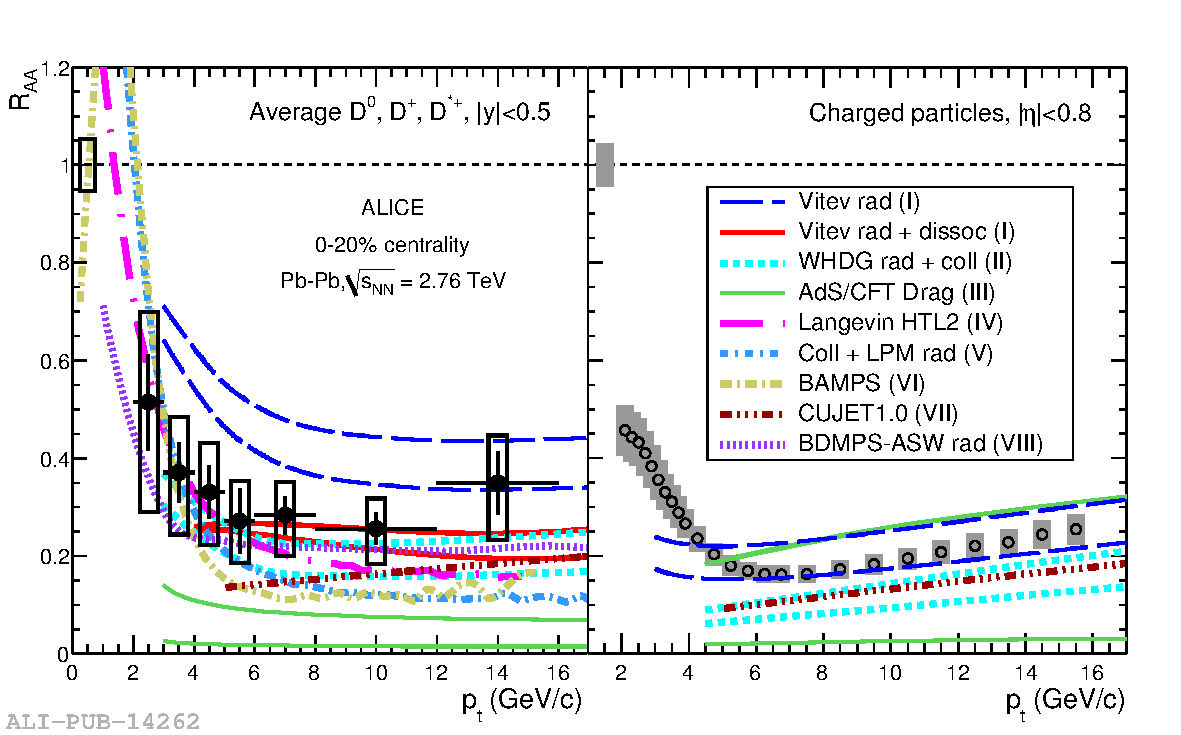
\includegraphics[width=0.7\textwidth]{ksfigures/DmesonChargedRAAmodels.pdf}
\caption{Average D-meson $R_{\rm AA}$ (left) and charged particle $R_{\rm AA}$ (right) as a function of $p_{\rm T}$ for the centrality between 0--20\,\%. The normalization uncertainties shown at unity in abscissa are almost fully correlated. The curves represent various model calculations, referred in the text, in some cases depicted as a range. Reproduced from~\cite{ALICE:2012ab}.}
\label{figks:DmesonRAA}
\end{figure}

Recently the family of measured D mesons was enlarged with the study of ${\rm D}_{\rm s}^+ \rightarrow {\rm K}^+{\rm K}^-\pi^+$ decay~\cite{Abelev:2012tca}. As a consequence of strangeness enhancement in heavy-ion collisions discussed in Sec.~\ref{subsecks:strangespectra}, the presence of strange quark may lead to a relative increase of ${\rm D}_{\rm s}$ production with respect to other D-mesons. Reported preliminary results show the ${\rm D}_{\rm s}$ $R_{\rm AA}$ in $p_{\rm T}$ region 4--12~GeV above the D-meson $R_{\rm AA}$, however, still within large uncertainties.

The behaviour of the charm-meson $R_{\rm AA}$ was confirmed by the measurement of the muon spectrum in the forward region $2.5 < y < 4$~\cite{Abelev:2012qh}. The contribution from pion and kaon decays is subtracted from the measured muon spectrum, and the results are presented for $p_{\rm T} > 4$~GeV, where this background contribution falls below 10\,\%. The obtained muon $p_{\rm T}$ spectrum thus represents a mixture of muons from semi-leptonic charm and beauty decays, presumably still dominated by charm at the lowest $p_{\rm T}$ and progressively becoming beauty dominated for $p_{\rm T} > 6$~GeV. An analogous  analysis of pp data is used for normalization, and the resulting heavy-flavour muon $R_{\rm AA}$ is presented in Fig.~\ref{figks:HFmuonRAA}. The muon $p_{\rm T}$, being correlated with the heavy-flavour-particle $p_{\rm T}$, is systematically smaller than the latter one (for $p_{\rm T}$ above a few GeV). Still, the comparison with the D-meson $R_{\rm AA}$ shows qualitative agreement, since the $p_{\rm T}$ dependence is rather flat. A similar measurement using electrons in mid-rapidity region was also reported~\cite{Abelev:2012xe}.

\begin{figure}
\centering
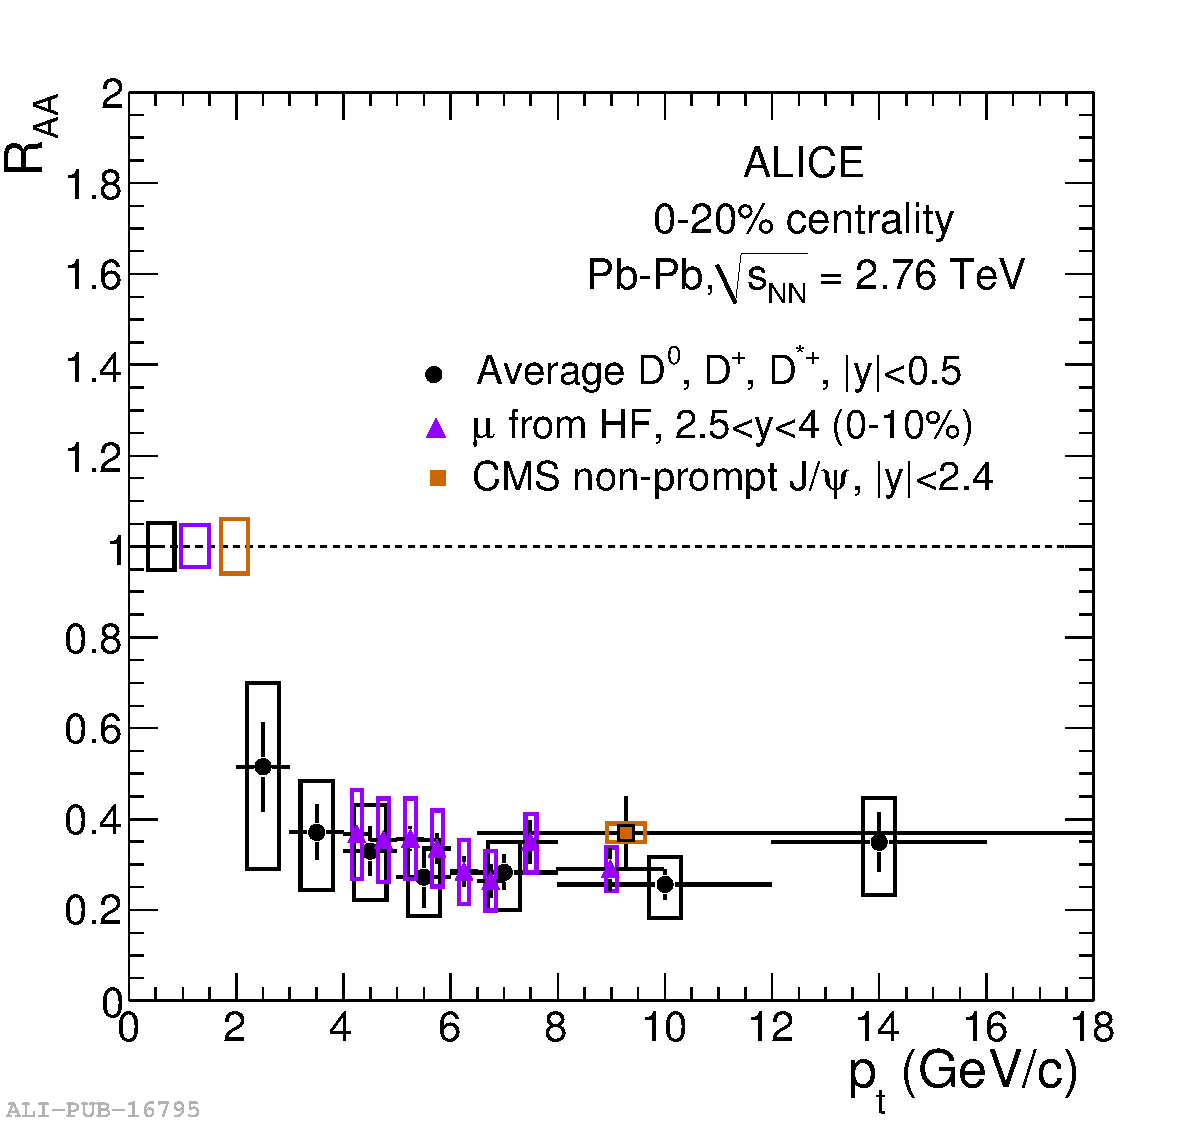
\includegraphics[width=0.5\textwidth]{ksfigures/DmesonHFmuonBRAA.pdf}
\caption{Heavy-flavour muon $R_{\rm AA}$ as a function of $p_{\rm T}$ compared to the average D-meson $R_{\rm AA}$. Results are for 0--20\,\% centrality class of Pb--Pb collisions. CMS preliminary result for beauty $R_{\rm AA}$ from measurement of non-prompt J/$\psi$ is shown with square. Reproduced from~\cite{Abelev:2012qh}.}
\label{figks:HFmuonRAA}
\end{figure}

In Fig.~\ref{figks:HFmuonRAA} the preliminary CMS result for $R_{\rm AA}$ from the measurement of non-prompt J/$\psi$ is shown~\cite{Chatrchyan:2012np}. The non-prompt J/$\psi$ particles are selected with careful analysis of the position of the J/$\psi$-decay point with respect to interaction vertex. These J/$\psi$'s are practically exclusively coming from B-meson decays. Recently reported detailed higher-statistics results on the centrality dependence of the $R_{\rm AA}$ for non-prompt J/$\psi$~\cite{CMS:2012wba} (in $p_{\rm T}$ range 6.5--30~GeV)  in comparison with the ALICE D-meson data (in $p_{\rm T}$ range 8--16~GeV) demonstrate clearly the larger $R_{\rm AA}$ for the beauty production than for the charm production, except for peripheral collisions, where the measurements are within their uncertainties. The shift between the $p_{\rm T}$ ranges takes into account that the J/$\psi$ momentum is lowered in the decay. This is for the first time that, as expected, the energy loss for beauty smaller than that for charm is experimentally observed.
%D-meson R_AA
%HF electron and muon R_AA
%Beauty suppression using B->J/psi+X
\subsection{Heavy-flavour elliptic flow}
\label{subsecks:heavyflow}
The primary cause of the elliptic azimuthal asymmetry is the asymmetric collision geometry: in semi-central collisions the overlapping region of the two nuclei has an almond shape, elongated in the direction perpendicular to the event plane (the plane defined by the beam axis and the centres of the colliding nuclei). The elliptic flow of charm was studied by the ALICE collaboration for D mesons using the event-plane method~\cite{Abelev:2013lca}. To estimate the azimuthal position of the event plane, charged tracks detected in the TPC are exploited. Then the yields of different D mesons are measured in the four azimuthal quadrants defined with respect to the event plane. From the yields in the two in-plane and in two out-of-plane quadrants the elliptic-flow coefficient $v_2$ is calculated. This is done independently for the three mesons: ${\rm D}^0$, ${\rm D}^+$, and ${\rm D}^{*+}$, and, as the $v_2$ values are compatible, they are then averaged applying beforehand the feed-down correction like in the case of the D-meson $R_{\rm AA}$. The $v_2$ results for the average D meson are presented in Fig.~\ref{figks:DmesonV2} for the centrality in the range 30--50\,\%. The comparison with the charged-particle $v_2$ obtained with the same method reveals a similar behaviour: the $v_2$ values for $p_{\rm T}$ between 2--8~GeV are compatible. This is the first direct observation of non-zero $v_2$ for a heavy-flavour particle. The large value of the charm $v_2$ at $p_{\rm T}$ around 2~GeV is interpreted as a signature of the in-medium thermalization of charm quarks.

\begin{figure}
\centering
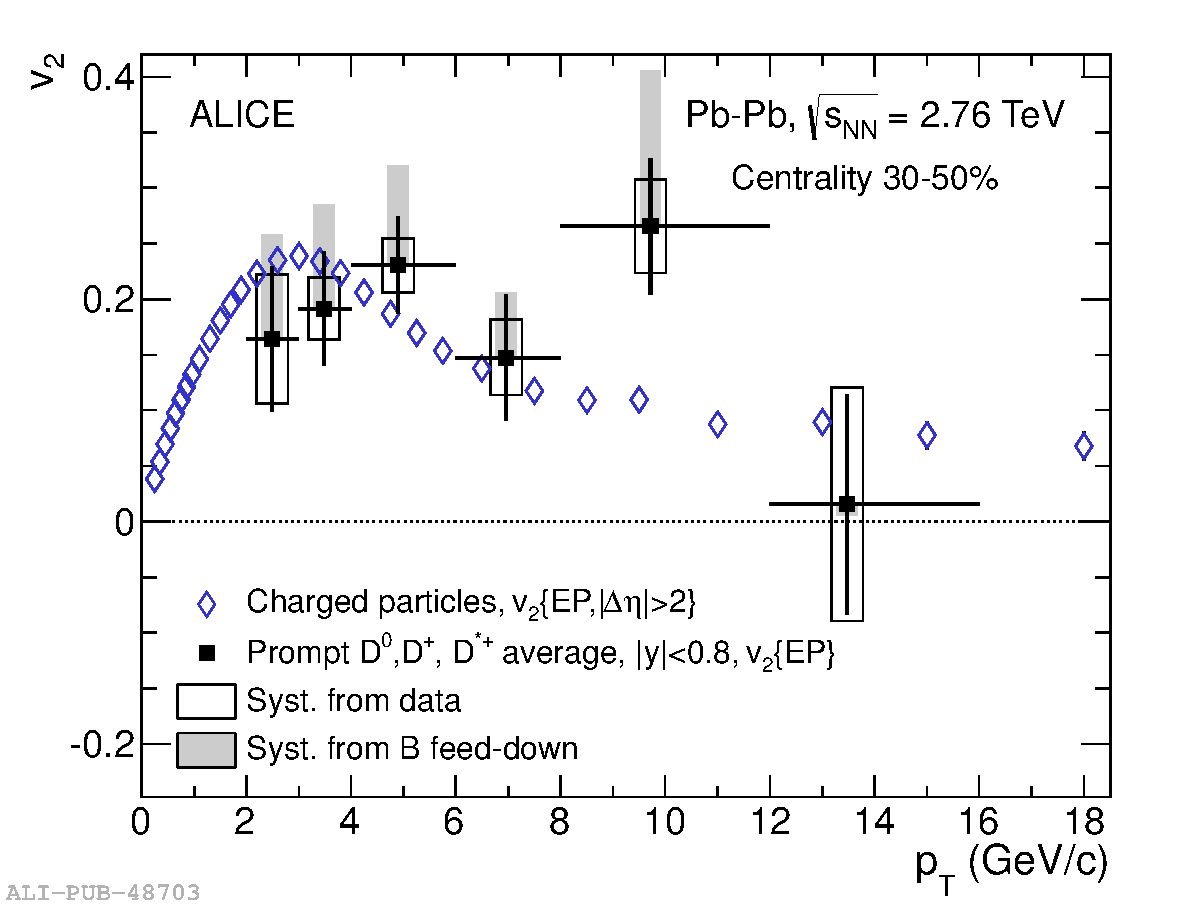
\includegraphics[width=0.5\textwidth]{ksfigures/DmesonV2.pdf}
\caption{Elliptic-flow coefficient $v_2$ obtained with the event-plane method, as a function of $p_{\rm T}$ for the centrality 30--50\,\%, averaged for ${\rm D}^0$, ${\rm D}^+$, and ${\rm D}^{*+}$, compared to the charged-particle measurement. Reproduced from~\cite{Abelev:2013lca}.}
\label{figks:DmesonV2}
\end{figure}

At higher $p_{\rm T}$ a positive $v_2$ can be generated by the difference in the in-medium path lengths for charm quarks emitted inside the in-plane azimuthal quadrants compared to those emitted in the out-of-plane quadrants. The shorter path length for the in-plane partons implies less suppression, i.e. larger $R_{\rm AA}$ for particles produced in this direction, than for those produced in the out-of-plane direction. In fact, the results can be presented as an azimuthally-dependent $R_{\rm AA}$, which is equivalent to the azimuthally-integrated $R_{\rm AA}$ and the $v_2$. The interpretation of the high-$p_{\rm T}$ $v_2$ as a path-length effect opens the possibility of studying  the in-medium path-length dependence of the parton energy loss.

The $v_2$ results for D mesons are complemented by the recently reported elliptic-flow measurements at forward rapidities ($2.5 < y < 4$) for the muons from heavy-flavour decays. They show an effect of similar magnitude. Indication of non-zero heavy-flavour $v_2$ using the semi-leptonic decays were previously published by RHIC experiments~\cite{Adler:2005ab,Adare:2006nq}.
%D-meson v2
%HF lepton v2
